\documentclass[12pt,a4paper]{article}
\usepackage{fontspec,xeCJK,amsmath,amssymb,graphicx,geometry,tabularx,array,booktabs,fancyhdr,titlesec,needspace,xurl}
\usepackage[unicode,hidelinks,bookmarksnumbered=false]{hyperref}
\geometry{left=28mm,right=28mm,top=25mm,bottom=25mm,headheight=20pt,headsep=7mm}
\setmainfont{Times New Roman}
\setsansfont{Arial}
\setCJKmainfont{SimSun}[AutoFakeBold=2.0]
\setCJKsansfont{SimHei}[AutoFakeBold=1.5]
\setCJKmonofont{SimSun}
\setmonofont{Arial}
\hypersetup{pdftitle={智储云控——基于决策导向预测融合的建筑储能削峰优化系统},pdfauthor={},pdfsubject={AI+能源 科技创新组技术报告},pdfcreator={XeLaTeX}}
\pagestyle{fancy}\fancyhf{}
\fancyhead[L]{\includegraphics[width=10mm]{qa/official_logo.png}}
\fancyhead[R]{\fontsize{9}{11}\selectfont 第八届全球校园人工智能算法精英大赛·算法主题赛}
\fancyfoot[C]{—\quad\thepage\quad—}
\renewcommand{\headrulewidth}{0.4pt}
\setlength{\parindent}{2em}\setlength{\parskip}{2pt}
\linespread{1}\raggedbottom
\setcounter{secnumdepth}{0}\setcounter{tocdepth}{2}
\renewcommand{\contentsname}{目录}
\titleformat{\section}{\sffamily\large\bfseries}{}{0pt}{}
\titleformat{\subsection}{\sffamily\normalsize\bfseries}{}{0pt}{}
\titleformat{\subsubsection}{\normalsize\bfseries}{}{0pt}{}
\titlespacing*{\section}{0pt}{15pt}{8pt}
\titlespacing*{\subsection}{0pt}{12pt}{6pt}
\titlespacing*{\subsubsection}{0pt}{10pt}{5pt}
\widowpenalty=10000\clubpenalty=10000
\emergencystretch=2em
\hbadness=10000
\begin{document}
\thispagestyle{fancy}
\vspace*{7mm}
\begin{center}
{\sffamily\fontsize{22}{30}\selectfont 2026 年第八届\\全球校园人工智能算法精英大赛\par}
\vspace{20mm}
{\sffamily\fontsize{22}{30}\selectfont 算法主题赛\\AI+能源\\技术报告\par}
\vspace{33mm}
\begin{minipage}{125mm}
\noindent 作品名称：{\sffamily\fontsize{20}{26}\selectfont 智储云控}\par\vspace{3mm}
\noindent {\fontsize{12}{20}\selectfont ——基于决策导向预测融合的\\建筑储能削峰优化系统}\par\vspace{6mm}
\noindent 赛道组别：科技创新组\par\vspace{6mm}
\noindent 团队名称：电协\par\vspace{6mm}
\noindent 团队编号：AIC-2026-27833449
\end{minipage}
\vfill
{\fontsize{16}{20}\selectfont 日期：2026 年 10 月 14 日}\vspace{24mm}
\end{center}
\clearpage

\phantomsection\section*{摘要}\addcontentsline{toc}{section}{摘要}
建筑侧储能的削峰效果不仅取决于负荷预测误差，还取决于误差出现的时段及电池可用能量。针对传统预测评价与储能调度目标不一致的问题，本作品提出决策导向预测融合方法 DOEF。该方法融合 LightGBM 与 DayWeek 周期预测，在验证集上以储能调度后悔值选择逐建筑权重，固定权重后开展测试。系统实现了历史负荷处理、预测训练、约束调度和多建筑结果回放。实验采用 BDG2 小时级用电数据，在固定的 8 栋办公建筑上开展对比与消融分析。相对 LightGBM，平均归一化 MAE 降低 6.36\%，平均归一化决策后悔值降低 3.61\%，6 栋改善、2 栋持平；平均整段削峰率为 6.44\%。与逐建筑 MAE 选权、全局决策选权相比，后悔值分别降低 12.48\% 和 3.17\%。结果支持以调度效果选择预测组合，并显示局部失效与样本依赖性。当前成果为离线仿真验证，结论限于本次建筑、测试月份和电池配置，可为建筑储能方案比较提供依据，现场经济与碳减排效益尚待验证。\par
关键词：人工智能；能源；建筑负荷预测；储能削峰；决策导向\par
\clearpage
\clearpage\tableofcontents\clearpage
\section{1. 项目背景与意义}
\subsection{1.1 能源行业痛点分析}
建筑电力负荷通常随人员活动和使用时段形成峰谷变化。对建筑侧储能而言，削峰的直接目标不是减少全天总用电量，而是在容量、功率、效率和荷电状态约束下压低最大电网取电功率。若高峰出现前的负荷预测失真，储能可能过早放电、在真正峰值到来时能量不足，或因错误充电形成新的峰值。因此，负荷预测只有通过调度动作和实际负荷共同评价，才能反映其对储能削峰的作用。\par
研究对象是 24 h 超前的小时级建筑负荷预测与日内电池削峰。历史负荷和预测时刻可获得的日历信息进入预测器，预测结果驱动 24 h 确定性储能优化；调度冻结后作用于实际负荷，再计算削峰和决策后悔值。该任务不涉及在线控制，也未模拟电价、碳排放或建筑总能耗变化。\par
在办公楼和校园办公区，楼宇能源管理人员需要提前安排储能电池的充放电。设想次日下午出现用电高峰，而电池电量有限：若预测把峰值时刻判断得过早，电池可能提前放电，在真正峰值到来时已没有足够电量。即使全天平均预测误差不大，削峰计划也可能失效。智储云控关注的是预测能否帮助使用者把有限电量留给关键时段，以降低建筑电网侧的最大取电功率。\par
这一场景用于解释工程需求，不是已部署案例。当前项目通过公开建筑数据完成离线预测、约束调度与结果评价，并用可视化原型支持方案比较；现场接入和运行收益仍待验证。\par
\subsection{1.2 人工智能技术应用价值}
MAE、RMSE 和平均绝对百分比误差（MAPE）是必要的预测评价指标，但它们将不同时刻的误差按固定规则汇总。储能削峰对误差位置并非同等敏感：峰值附近的负荷高低和时序判断会改变充放电计划，而部分低谷误差可能对当日最大需量影响有限。因而，“预测误差更小”与“调度后的实际峰值更低”在本项目中不是同一命题。\par
八建筑测试集提供了一个范围明确的反例：XGBoost 的平均归一化 RMSE 为 0.216751，略低于 LightGBM 的 0.216942，但其平均归一化决策后悔值为 0.117534，高于 LightGBM 的 0.116127（图 1）。两组差距均较小，该结果只说明在本项目的固定样本和调度协议内，预测排序不能完全代替决策排序；它不支持“预测精度不重要”或普适因果结论。\par
\par\noindent\begin{minipage}{\linewidth}\centering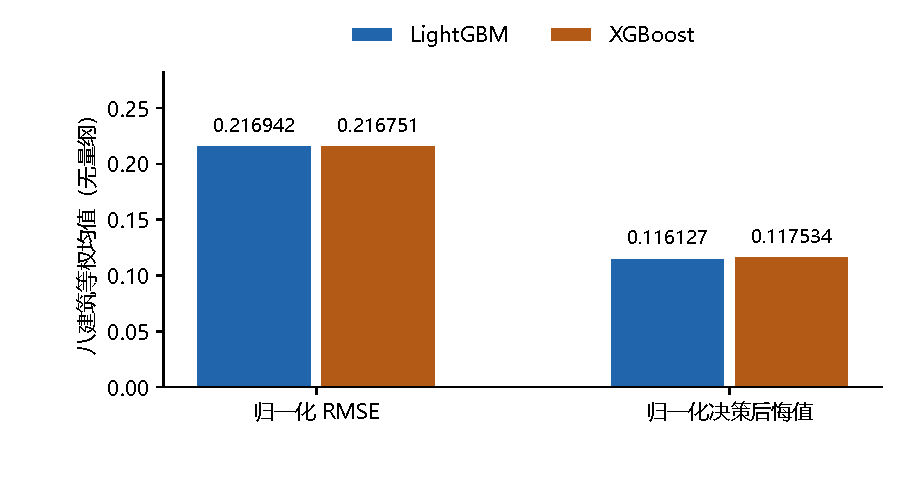
\includegraphics[width=\linewidth]{figures/mismatch.pdf}\par\raggedright \textbf{图 1｜预测指标不能单独决定储能决策价值。} 图中比较八建筑测试集等权聚合结果。XGBoost 的归一化 RMSE 略低，但归一化决策后悔值略高，表明两类指标在该实验范围内可能给出不同排序。\par\end{minipage}\par
建筑负荷预测研究已经比较了多类回归和机器学习模型[2,3]，部分工作也把负荷或峰值预测接入建筑、园区及电池储能优化[4-8]。predict-then-optimize 和 decision-focused learning 研究进一步讨论预测损失与下游目标的偏离，并提出任务损失训练或决策导向的模型选择方法[9-11]。DOEF 同样主张按下游用途评价预测，但实现范围较窄：它既不进行端到端训练，也不学习新的优化器，而是在已有 DayWeek 与 LightGBM 预测之间，用验证集储能决策后悔值选择逐建筑固定权重。已有决策导向预测组合研究已经利用下游目标选择组合权重[12]。DOEF 的具体贡献是将该思想用于建筑负荷点预测与固定电池削峰：以各建筑验证集上的实际调度后悔值，在 DayWeek-LightGBM 两分量的有限网格中选择权重，冻结后用于测试。该贡献属于应用方法改进，不声称首次提出决策导向组合，不包括 LightGBM、滞后特征或通用削峰优化本身。\par
\subsection{1.3 项目目标与意义}
给定建筑 \(b\) 在预测时刻可获得的信息，预测未来 24 个小时的负荷 \(\hat{y}_{b,t}\)。预测层报告 MAE、RMSE、MAPE 及按训练期平均负荷归一化的指标；决策层以预测负荷生成电池充放电计划，并用实际负荷计算调度后的峰值、削峰率和相对 Oracle 的决策后悔值。项目目标是依据验证集调度表现选择预测融合权重，并在冻结的留出评价期检验储能削峰效果；历史方法路线筛选的边界见 3.3.6 节。\par
\section{2. 技术方案与实现}
\subsection{2.1 总体架构设计}
智储云控由离线实验计算与结果展示两部分组成。计算端依次执行数据质量控制、因果特征构造、逐建筑模型训练、验证集权重选择及固定约束下的储能调度；展示端读取已经保存的实验结果，供用户比较建筑、预测方法和削峰效果。验证集用于选模，测试期实际负荷仅在调度计划冻结后用于评价，不进入预测或调度求解。\par
数据处理、预测训练、权重选择、电池优化和结果展示按模块实现；各模块通过统一的数据字段交换预测、配置和调度结果。浏览器界面提供本地服务与离线 HTML 两种访问方式。\par
\par\noindent\begin{minipage}{\linewidth}\centering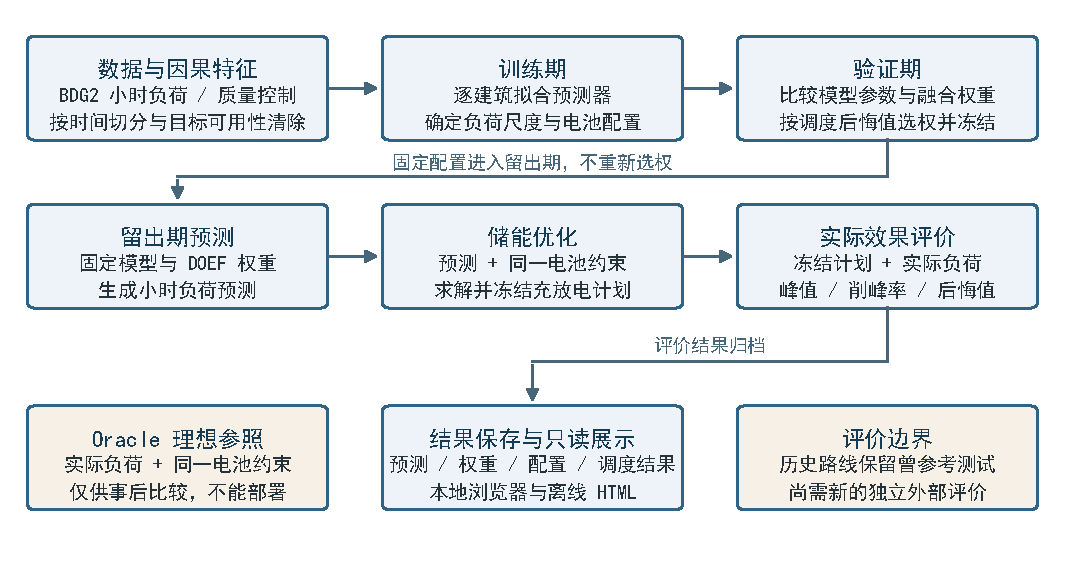
\includegraphics[width=\linewidth]{figures/architecture.pdf}\par\raggedright \textbf{图 2｜离线计算与展示架构。} 训练期用于模型拟合、建筑尺度统计与电池配置；验证期用于模型参数及融合权重选择；测试预测形成冻结调度计划，随后结合实际负荷评价。Oracle 使用实际负荷求解同约束理想参照，不能部署。展示端只读保存结果。图示为冻结配置的计算流程，历史方法路线筛选另见 3.3.6 节。\par\end{minipage}\par
\subsection{2.2 核心算法与模型}
\subsubsection{2.2.1 周期基线与 LightGBM}
表 1 给出实际使用的预测基线。项目早期材料中的 Persistence 与 Day 是同一科学方法，不作为两个独立基线重复计数。DayWeek 是固定周期平均，不含学习参数。\par
\par\noindent\begin{minipage}{\linewidth}\textbf{表 1｜预测方法及其定义}\par\smallskip\renewcommand{\arraystretch}{1.2}\begin{tabularx}{\linewidth}{>{\hsize=0.65\hsize\linewidth=\hsize\raggedright\arraybackslash}X>{\hsize=1.35\hsize\linewidth=\hsize\raggedright\arraybackslash}X}\toprule
方法 & 定义或作用\\\midrule
Day Persistence & \(\hat{y}_t=y_{t-24}\)，沿用前一日同小时实际负荷\\
Week & \(\hat{y}_t=y_{t-168}\)，沿用前一周同小时实际负荷\\
DayWeek & \(\hat{y}_t=0.5y_{t-24}+0.5y_{t-168}\)\\
LightGBM & 逐建筑训练的梯度提升树预测器\\
XGBoost / CatBoost & 冻结对比模型\\
DOEF & DayWeek 与 LightGBM 的验证集决策导向融合\\
\bottomrule\end{tabularx}\end{minipage}\par
LightGBM 能处理非线性关系、离散日历状态和多尺度滞后特征，训练与推理开销也较低。输入包括当前特征时刻的负荷、日历编码、1/2/3/24/48/72/168/336 h 正滞后，以及先移位后计算的滚动统计。所有特征在预测时刻均可获得；项目没有使用未来目标或未来天气，也没有加入天气、节假日等外部数据。每栋建筑的候选参数和验证集选择结果均记录在冻结配置中。LightGBM 是基础预测器，并非本项目原创算法。\par
\subsubsection{2.2.2 储能削峰优化模型}
每栋建筑使用按训练期平均日用电量缩放的独立电池，但所有预测方法共享该建筑的同一配置。名义容量为训练期平均日用电量的 10\%，最大充电与放电功率均为容量的 25\%/h。SOC 范围为 10\% 至 90\%，每天初始和终止 SOC 均为 50\%。充、放电效率均为 \(\sqrt{0.9}\)，往返效率为 90\%。表 2 汇总共同规则；逐建筑容量从 20.507 kWh 到 2,857.763 kWh，完整数值由冻结配置给出。\par
\par\noindent\begin{minipage}{\linewidth}\textbf{表 2｜电池共同参数}\par\smallskip\renewcommand{\arraystretch}{1.2}\begin{tabularx}{\linewidth}{>{\raggedright\arraybackslash}X>{\raggedright\arraybackslash}X}\toprule
参数 & 取值\\\midrule
容量规则 & 训练期平均日用电量的 10\%\\
最大充电功率 & 容量的 25\%/h\\
最大放电功率 & 容量的 25\%/h\\
SOC 下限 / 上限 & 10\% / 90\%\\
日初 / 日末 SOC & 50\% / 50\%\\
充电效率 / 放电效率 & 0.948683 / 0.948683\\
往返效率 & 0.90\\
调度周期 & 24 h，每日重置\\
\bottomrule\end{tabularx}\end{minipage}\par
对每个 24 h 调度日，令 \(c_t\ge 0\) 和 \(d_t\ge 0\) 分别为充电、放电功率，\(s_t\) 为 SOC，\(z_t\in\{0,1\}\) 为互斥模式变量，\(p^{\max}\) 为预测负荷下的目标峰值。冻结实现求解：\par
\[
\min \; p^{\max}+\epsilon\sum_{t=1}^{24}(c_t+d_t),
\qquad \epsilon=10^{-6},
\]
并满足\par
\[
\hat{y}_t+c_t-d_t\le p^{\max},
\]
\[
s_{t+1}=s_t+\eta_c c_t-\frac{d_t}{\eta_d},
\]
\[
s^{\min}\le s_t\le s^{\max},\quad
0\le c_t\le z_t P_c^{\max},\quad
0\le d_t\le (1-z_t)P_d^{\max},
\]
\[
s_1=s_{25}=0.5C.
\]
该混合整数线性规划由 \nolinkurl{scipy.optimize.milp} 求解。调度阶段只读取预测负荷，实际未来负荷不参与求解；实际负荷仅在计划冻结后用于计算实现峰值。Oracle 以实际负荷求解同一问题，只作为不可部署的评价参照。\par
\subsubsection{2.2.3 决策导向预测融合}
预测误差会先改变电池计划，再影响实际峰值，并不直接等同于决策误差。低估峰值时段可能使优化器预留不足；高估错误时段则可能把有限能量用在非关键时段。因此，两种预测即使整体 MAE 或 RMSE 接近，也可能因为峰值时序不同而生成不同的充放电轨迹。\par
图 1 的 XGBoost-LightGBM 排序反例说明这种差异确实出现在冻结实验中。验证阶段进一步显示，若分别以 MAE 和决策后悔值选择同一组候选融合权重，8 栋建筑中有 6 栋得到不同权重（图 3）。这两项证据共同支持双层评价：预测指标用于检查基本拟合质量，决策指标用于评价预测进入储能优化后的任务价值。\par
该观察不等同于“峰值附近误差必然导致更差调度”。本项目的结果是由既定电池参数、每日 SOC 重置和确定性峰值目标共同产生；改变电池规模、动态电价或控制时域可能改变误差与决策的关系。\par
DOEF v1.0 使用两个已有预测分量：DayWeek 提供稳定的日周周期参照，LightGBM 表达逐建筑的非线性负荷规律。对建筑 \(b\)，最终预测为：\par
\[
\hat{y}_{b,t}^{\text{DOEF}}
=w_b\hat{y}_{b,t}^{\text{LightGBM}}
+(1-w_b)\hat{y}_{b,t}^{\text{DayWeek}},
\qquad w_b\in\{0.0,0.1,\ldots,1.0\}.
\]
DOEF 不是简单平均：权重随建筑变化，并由验证集下游决策目标选择。它也不是端到端学习，因为预测器参数与储能优化器没有联合训练，决策目标只用于选择冻结候选权重。\par
\subsubsection{2.2.4 验证集权重选择}
对每个候选 \(w_b\)，系统先在验证集形成融合预测，再用相同电池约束逐日求解调度，并计算相对 Oracle 的平均日决策后悔值。权重按冻结的等价带和平局规则选择；候选集合、评价目标和规则均在测试前确定。选定后，\(w_b\) 固定转移到测试集，不再更新。\par
\par\noindent\begin{minipage}{\linewidth}\textbf{表 3｜逐建筑冻结融合权重}\par\smallskip\renewcommand{\arraystretch}{1.2}\begin{tabularx}{\linewidth}{>{\hsize=1.4\hsize\linewidth=\hsize\raggedright\arraybackslash}X>{\hsize=0.8\hsize\linewidth=\hsize\raggedright\arraybackslash}X>{\hsize=0.8\hsize\linewidth=\hsize\raggedright\arraybackslash}X}\toprule
建筑 & MAE 选择的 LightGBM 权重 & 决策后悔值选择的 LightGBM 权重（DOEF）\\\midrule
Hog\_office\_Rolando & 0.9 & 0.7\\
Hog\_office\_Lavon & 0.0 & 0.0\\
Hog\_office\_Joey & 0.6 & 0.3\\
Lamb\_office\_Caitlin & 0.4 & 0.8\\
Robin\_office\_Addie & 1.0 & 1.0\\
Lamb\_office\_Gerardo & 0.0 & 1.0\\
Hog\_office\_Alexis & 0.6 & 0.7\\
Hog\_office\_Byron & 0.9 & 0.8\\
\bottomrule\end{tabularx}\end{minipage}\par
\par\noindent\begin{minipage}{\linewidth}\centering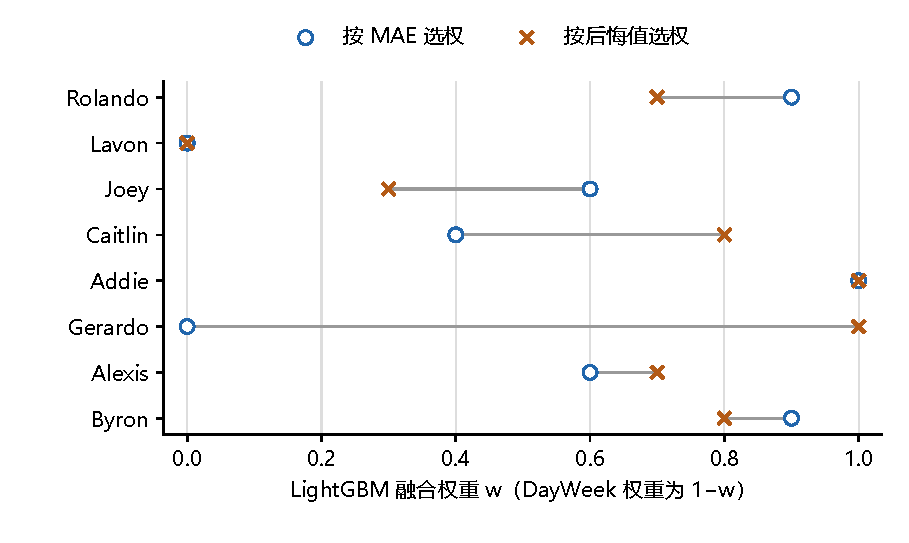
\includegraphics[width=\linewidth]{figures/weights.pdf}\par\raggedright \textbf{图 3｜验证集融合权重选择。} MAE 最优权重与决策后悔值最优权重在 6 栋建筑上不同。测试集不参与权重或平局规则选择，图中展示验证结束后固定的权重。\par\end{minipage}\par
常见流程用验证集 MAE 或 RMSE 选定预测模型，再把预测直接输入优化器。DOEF 仍遵守相同的数据隔离原则，但权重依据验证集下游储能决策后悔值选择。这是一种任务导向的选择关系，不是可微的端到端训练。方法结构透明、便于复核，其能力也受到两个固定预测分量和离散权重网格的限制。\par
\subsection{2.3 数据处理与分析}
\subsubsection{2.3.1 数据来源与单位}
实验使用 BDG2 的 \nolinkurl{electricity_cleaned.csv} 与 \nolinkurl{metadata.csv}[1]。数据下载来源、许可及署名说明见随包 \nolinkurl{docs/DATASET.md}；第三方数据和基础算法的权益归原作者，本文的原创贡献范围见 4.1 节。原始电表读数的语义是每小时区间的电能 \(E_t\)（kWh）。调度按 \(\Delta t=1\,\text{h}\) 将其解释为区间平均功率：\par
\[
P_t = \frac{E_t}{\Delta t}.
\]
因此数值在一小时时间步下相同，但负荷和充放电功率使用 kW，电池容量与 SOC 使用 kWh，两种单位在语义上不可互换。\par
\subsubsection{2.3.2 建筑筛选与质量控制}
建筑选择表包含 1,578 条建筑序列，其中 296 条为办公建筑候选，82 条通过确定性覆盖与质量规则。最终 8 栋建筑由一栋既定锚点建筑与训练期负荷形态空间中的确定性最远点采样组成。形态特征包括负荷规模、变异系数、峰均比、峰谷差、24 h 与 168 h 自相关、工作日和周末差异、日曲线变异及稳健异常比例。验证集或测试集上的预测、调度成绩均未参与选楼。\par
这种选择方式避免用测试成绩挑选建筑，但不能据此声称模型能够迁移到未见建筑。报告中的“多建筑稳健性”仅指 8 栋预先固定办公建筑上的一致性评价。\par
\subsubsection{2.3.3 因果时间切分}
特征时刻的锚定时间窗见表 4。目标由固定 24 h 前视位移形成，边界处执行目标可用性清除，避免训练或验证样本引用后续区间的目标值。每栋建筑的测试集包含 720 个小时目标，即 30 个完整调度日。\par
\par\noindent\begin{minipage}{\linewidth}\textbf{表 4｜数据切分与用途}\par\smallskip\renewcommand{\arraystretch}{1.2}\begin{tabularx}{\linewidth}{>{\hsize=0.55\hsize\linewidth=\hsize\raggedright\arraybackslash}X>{\hsize=1.1\hsize\linewidth=\hsize\raggedright\arraybackslash}X>{\hsize=1.55\hsize\linewidth=\hsize\raggedright\arraybackslash}X>{\hsize=0.8\hsize\linewidth=\hsize\raggedright\arraybackslash}X}\toprule
数据分区 & 特征时刻范围 & 主要用途 & 是否参与最终报告评价\\\midrule
训练集 & 2016-01-15 至 2017-10-31 & 特征统计、基础模型训练、电池按训练期尺度配置 & 否\\
验证集 & 2017-11-01 至 2017-11-30 & 基础模型与 DOEF 权重选择、平局规则执行 & 否\\
测试集 & 2017-12-01 至 2017-12-30 & 冻结算法的最终评价 & 是\\
\bottomrule\end{tabularx}\end{minipage}\par
建筑筛选与已登记参数、融合权重的搜索未使用测试成绩。历史阶段已经查看过测试结果，且最终方法路线的保留参考过冻结测试证据，因此本报告称其为“冻结的留出评价期”，不称为未参与开发判断的全新盲测集。参数选择与方法路线保留应分别理解，具体边界见 3.3.6 节。\par
\subsection{2.4 系统功能实现}
系统提供八建筑巡演与综合结果两个主要视图。巡演视图随回放进度更新建筑和日期，展示无储能、LightGBM 与 DOEF 对应的每日取电峰值曲线，并同步显示所选建筑的电池配置和结果指标。开始巡演后，界面依次回放各建筑；用户可暂停、继续或切换至下一栋，综合结果在八建筑巡演结束后显示。综合结果视图展示逐建筑比较与等权聚合指标，保留负削峰案例。\par
用户可直接打开随包的离线 HTML，无需联网或安装依赖；也可在源码目录执行 \texttt{python gui/server.py}，在浏览器访问 \nolinkurl{http://127.0.0.1:8765}。该服务仅依赖 Python 标准库。现有功能支持查看和比较已完成的实验，尚不支持上传任意建筑数据后自动训练，也未接入现场电池控制接口。\par
\section{3. 实验结果与分析}
\subsection{3.1 实验环境与设置}
实验环境如下：最终算法验证记录的处理器标识为 Intel64 Family 6 Model 186 Stepping 2, GenuineIntel，架构为 AMD64，系统标识为 Windows-10-10.0.26200-SP0，Python 为 3.11.9。pandas 版本为 2.3.3。上述为原实验记录，原运行内存容量及 NumPy、SciPy、LightGBM 等确切版本未保存，不能用当前安装版本代替原始记录。随包 requirements.txt 给出依赖范围，docs/REPRODUCING.md 给出数据获取和分阶段执行步骤。\par
2026 年 10 月 13 日的材料复核环境另行记录：Python 3.12.14、pandas 2.3.3、NumPy 2.5.2、SciPy 1.18.1、scikit-learn 1.9.0、LightGBM 4.7.0、XGBoost 3.2.0、CatBoost 1.2.10、Matplotlib 3.11.1，当前主机物理内存约 15.64 GiB。该环境用于文稿生成、冻结结果核对及材料一致性检查，未据此重新训练模型或执行调度，不能视为完整重训复现证明。详细记录见随包 reports/provincial\_20261012/report\_revision.json。\par
核心模型采用 CPU 训练，随机种子为 42，线程数为 4。多建筑树模型的最大训练预算为 500 棵树，学习率为 0.03，早停耐心为 50 轮。LightGBM 比较平衡型和小规模正则化两组参数：叶子数分别为 31 和 15，最大深度分别为不限和 6，最小叶样本数分别为 20 和 30，L2 正则项分别为 0 和 0.2；行、列采样比例均为 0.8。逐建筑参数及最佳迭代数保存在模型配置中。既定锚点建筑的兼容预测按原冻结来源复用，其训练来源与新建多建筑模型分别记录。\par
储能优化使用 SciPy 的混合整数线性规划接口，电池容量、效率、SOC 和日末约束沿用前文设置。模型参数与融合权重分别在验证集上确定；测试集不用于追加搜索。包内提供依赖安装、原始数据获取和分阶段执行说明。保存的预测与调度结果可直接复核；完整重训需获取原始数据并按环境说明执行。\par
\subsection{3.2 评价指标}
设测试样本数为 \(n\)，实际负荷为 \(y_i\)，预测负荷为 \(\hat{y}_i\)，则：\par
\[
\mathrm{MAE}=\frac{1}{n}\sum_{i=1}^{n}|y_i-\hat{y}_i|,
\qquad
\mathrm{RMSE}=\sqrt{\frac{1}{n}\sum_{i=1}^{n}(y_i-\hat{y}_i)^2},
\]
\[
\mathrm{MAPE}=\frac{100\%}{|\mathcal I|}\sum_{i\in\mathcal I}\left|\frac{y_i-\hat{y}_i}{y_i}\right|,
\qquad \mathcal I=\{i:|y_i|>10^{-12}\}.
\]
跨建筑主比较采用各建筑指标除以对应训练期平均负荷后的等权平均，以免大负荷建筑仅因量级主导结果。MAPE 对接近零负荷敏感，因此作为补充指标，不用于支持核心排序结论。\par
实现电网负荷为 \(g_t=y_t+c_t-d_t\)。整段削峰率定义为：\par
\[
r_{\text{peak}}=\frac{\max_t y_t-\max_t g_t}{\max_t y_t}\times100\%.
\]
某日的决策后悔值定义为预测驱动计划的实际日峰值与 Oracle 实际日峰值之差：\par
\[
R_d=\max_{t\in d}g_t^{\text{method}}-\max_{t\in d}g_t^{\text{Oracle}}.
\]
后悔值的单位为 kW；归一化后除以该建筑训练期平均负荷。它不是电费、收益或碳排放意义上的“后悔”。\par
\subsection{3.3 结果展示与分析}
\subsubsection{3.3.1 预测性能}
表 5 报告冻结测试集的八建筑等权聚合结果。DOEF 的平均归一化 MAE 与 RMSE 在所列方法中最低，分别为 0.137970 和 0.207822。LightGBM 的归一化 MAE 为 0.147338，低于 DayWeek 的 0.183478，但 XGBoost 的归一化 RMSE 以 0.216751 略低于 LightGBM 的 0.216942。不同模型在局部指标上各有优势。MAPE 在低负荷建筑上容易放大，因此不作为跨建筑主结论的依据。\par
\par\noindent\begin{minipage}{\linewidth}\textbf{表 5｜测试集预测层聚合结果}\par\smallskip\renewcommand{\arraystretch}{1.2}\begin{tabularx}{\linewidth}{>{\hsize=1.4\hsize\linewidth=\hsize\raggedright\arraybackslash}X>{\hsize=0.8666666666666667\hsize\linewidth=\hsize\raggedright\arraybackslash}X>{\hsize=0.8666666666666667\hsize\linewidth=\hsize\raggedright\arraybackslash}X>{\hsize=0.8666666666666667\hsize\linewidth=\hsize\raggedright\arraybackslash}X}\toprule
方法 & 平均归一化 MAE & 平均归一化 RMSE & 平均 MAPE（\%）\\\midrule
Day Persistence & 0.225885 & 0.430193 & 21.33\\
Week & 0.201578 & 0.328414 & 23.52\\
DayWeek & 0.183478 & 0.296621 & 20.03\\
LightGBM & 0.147338 & 0.216942 & 30.90\\
XGBoost & 0.149781 & 0.216751 & 32.48\\
CatBoost & 0.173604 & 0.239211 & 33.14\\
DOEF & 0.137970 & 0.207822 & 16.20\\
\bottomrule\end{tabularx}\end{minipage}\par
\subsubsection{3.3.2 削峰决策效果}
相对 LightGBM，DOEF 的平均归一化 MAE 从 0.147338 降至 0.137970，相对改善 6.3585\%；平均归一化决策后悔值从 0.116127 降至 0.111929，相对改善 3.6147\%（图 4）。建筑级决策后悔值比较为 6 胜、2 平、0 负。以建筑为重采样单位的 10,000 次 bootstrap 给出 DOEF 减 LightGBM 的平均归一化后悔值差为 -0.004198，95\% 区间为 [-0.006850, -0.001719]。该区间描述本次 8 栋建筑样本内的不确定性，外部适用性仍需更多建筑验证。\par
\par\noindent\begin{minipage}{\linewidth}\centering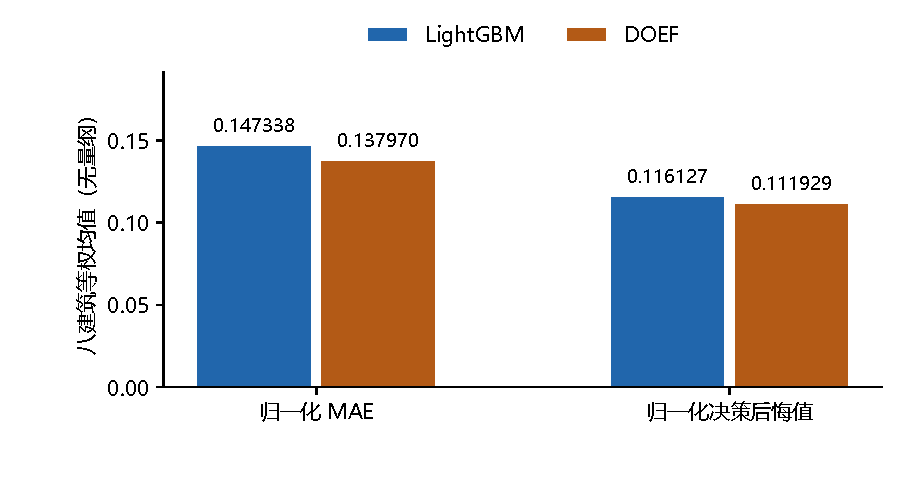
\includegraphics[width=\linewidth]{figures/main_results.pdf}\par\raggedright \textbf{图 4｜DOEF 的实验主结果。} 在八建筑测试集等权聚合下，DOEF 相对 LightGBM 同时降低平均归一化 MAE 和平均归一化决策后悔值。两项指标均先按训练期平均负荷归一化，再对全部八建筑等权平均；削峰率统计及负值案例见本节后续正文。\par\end{minipage}\par
整段削峰率提供不同于后悔值的工程视角。DOEF 的平均值为 6.4423\%，中位数为 5.6291\%，最小值为 -1.0170\%，最大值为 14.0162\%。最小值为负，说明至少一栋建筑在测试期出现反向削峰，即调度后的实际最大负荷高于原始负荷峰值。CatBoost 的最小削峰率为 -245.9433\%，反映了预测偏差可能造成的严重调度失效。\par
对比实验还记录了稳健调度的失效案例。在锚点建筑测试中，验证集选择的稳健调度平均后悔值为 20.4635 kW，高于确定性 LightGBM 调度的 11.1274 kW，该结果不支持此稳健配置改善本次削峰表现，仅作为历史负结果保留，不推断稳健优化普遍无效。峰值加权 LightGBM 也作为支持性实验保留；最终方法路线与测试证据的关系见 3.3.6 节。\par
\subsubsection{3.3.3 建筑间结果差异}
图 5 按冻结选择顺序展示全部 8 栋建筑。DOEF 在 6 栋建筑上的平均归一化决策后悔值低于 LightGBM，在 2 栋上因 DOEF 的冻结 LightGBM 权重为 1.0 而与 LightGBM 持平。该比较包含全部建筑，评价范围为预先固定的办公建筑及一个未来测试月。\par
\par\noindent\begin{minipage}{\linewidth}\centering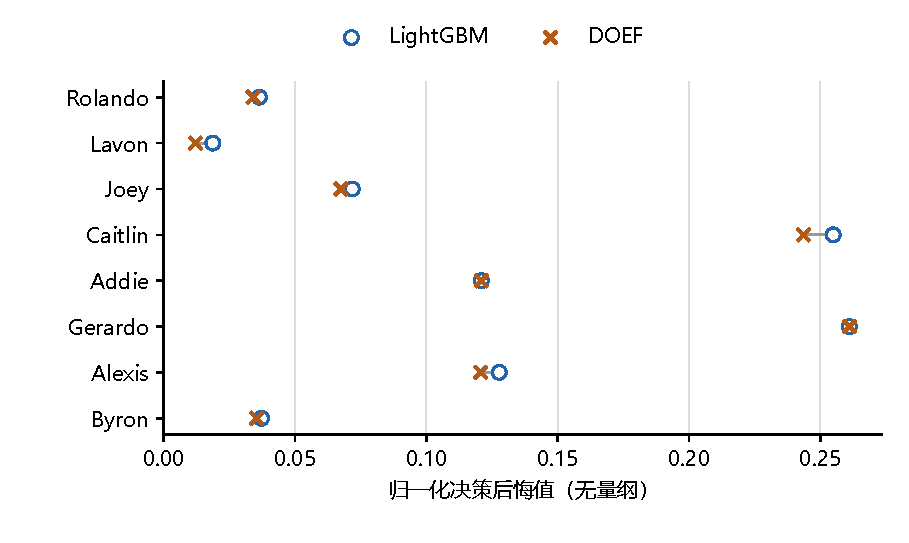
\includegraphics[width=\linewidth]{figures/buildings.pdf}\par\raggedright \textbf{图 5｜八栋固定建筑的决策价值比较。} 每个点是建筑测试期平均日决策后悔值除以该建筑训练期平均负荷。该图支持多建筑稳健性，不支持未见建筑、其他季节或跨年份迁移。\par\end{minipage}\par
\subsubsection{3.3.4 选权目标与逐建筑适配消融}
各方案使用相同预测分量、测试期和电池约束；单分量对照对应融合权重端点。全局 MAE 选权的验证集最优权重为 0.5，因此其测试结果与等权融合相同。\par
\par\noindent\begin{minipage}{\linewidth}\textbf{表 6｜冻结测试集中的选权对照}\par\smallskip\renewcommand{\arraystretch}{1.2}\begin{tabularx}{\linewidth}{>{\hsize=1.4\hsize\linewidth=\hsize\raggedright\arraybackslash}X>{\hsize=0.8\hsize\linewidth=\hsize\raggedright\arraybackslash}X>{\hsize=0.8\hsize\linewidth=\hsize\raggedright\arraybackslash}X}\toprule
方法 & 平均归一化 MAE & 平均归一化后悔值\\\midrule
仅 DayWeek（w=0） & 0.183478 & 0.143019\\
仅 LightGBM（w=1） & 0.147338 & 0.116127\\
等权融合（w=0.5） & 0.151790 & 0.125230\\
逐楼按 MAE 选权 & 0.168297 & 0.127887\\
全局决策选权（w=0.8） & 0.143470 & 0.115591\\
DOEF：逐楼按后悔值选权 & 0.137970 & 0.111929\\
\bottomrule\end{tabularx}\end{minipage}\par
在保持逐建筑选权的条件下，将选择目标从验证集 MAE 改为验证集调度后悔值，测试期平均归一化后悔值由 0.127887 降至 0.111929，相对降低 12.48\%，建筑级比较为 5 胜、2 平、1 负。该对照直接检验选权目标的作用，比较对象是逐楼 MAE 选权，相对 LightGBM 的结果见决策层比较。\par
在保持决策选权目标的条件下，相对全局共用权重 w=0.8 的方案，DOEF 的平均归一化后悔值由 0.115591 降至 0.111929，相对降低 3.17\%，建筑级比较为 6 胜、2 平、0 负。该结果支持本样本中逐建筑适配的增益，不代表任何逐楼选权方式均优于全局选择。上述百分比从未舍入结果计算。\par
\subsubsection{3.3.5 样本依赖性与失效案例}
为考察样本依赖性，对固定逐建筑指标进行留一建筑汇总；模型与权重保持不变。以逐楼 MAE 选权为基线，Gerardo 贡献了八建筑归一化后悔值总差额的约 82.44\%。仅将 Gerardo 从均值汇总中移除，剩余建筑的相对改善为 3.41\%；依次移除每一栋建筑，改善范围为 3.41\%–14.22\%。这表明方向不完全依赖单栋建筑，但收益幅度具有明显样本依赖性；该分析反映样本构成的影响，不构成独立外部验证。\par
单日失效案例来自同一批既有调度结果：Joey 在 2017-12-14 的无储能峰值为 1446.768000 kW，逐楼 MAE 选权方案为 1332.581714 kW，DOEF 为 1380.125054 kW，Oracle 为 1309.840231 kW；DOEF 比 MAE 选权高 47.543340 kW。案例按两种选权策略在测试日的峰值差绝对值最大事后选取，不是预先指定。该日两种方案均优于无储能，与该楼整月负削峰率是不同事实；具体失效机制仍需结合逐时调度轨迹分析。\par
\subsubsection{3.3.6 评价协议}
DOEF 的候选权重按“验证集选择、权重冻结、留出期评价”的顺序计算。图 3 展示验证集上两种目标对应的固定权重，不含测试期权重优化。这里的参数搜索隔离不等于整个方法开发过程未参考测试结果。\par
历史记录显示，多建筑融合方案的保留及峰值加权方案的最终晋级判断曾参考冻结测试表现。因而，本报告的比较属于既有开发过程中的留出期证据，不能作为完全独立于方法路线选择的盲测证明；样本内置信区间也不消除这种选择影响。报告保留全部固定建筑、负结果及失效案例，不追加测试期调参。进一步确认泛化收益，需要先锁定完整方法路线，再在未用于开发的新月份或新建筑上评价。\par
\subsubsection{3.3.7 结果一致性与可复现性}
用显式 DOEF 公式、固定分量预测和决策选权重建测试预测，并与保存的参考预测逐点比较。8 栋建筑共 5,760 个预测值的最大绝对差为 0.0 kW，容差为 \(10^{-12}\)。同时，共 76 个登记实验文件通过 LF 归一化哈希审计。复核过程中未改变模型、权重或测试样本。\par
\par\noindent\begin{minipage}{\linewidth}\textbf{表 7｜预测一致性与文件完整性检查}\par\smallskip\renewcommand{\arraystretch}{1.2}\begin{tabularx}{\linewidth}{>{\hsize=1.4\hsize\linewidth=\hsize\raggedright\arraybackslash}X>{\hsize=0.8\hsize\linewidth=\hsize\raggedright\arraybackslash}X>{\hsize=0.8\hsize\linewidth=\hsize\raggedright\arraybackslash}X}\toprule
检查对象 & 规模 & 结果\\\midrule
DOEF 测试预测逐点一致性 & 8 栋 × 720 h = 5,760 点 & 最大绝对差 0.0 kW，PASS\\
实验文件哈希 & 76 个文件 & 76/76 PASS\\
DOEF 候选权重选择数据源 & 验证集 & PASS\\
留出期使用边界 & 冻结权重评价；历史路线保留曾参考测试 & 已披露\\
约束审计 & 同一冻结电池与优化器 & PASS\\
\bottomrule\end{tabularx}\end{minipage}\par
\clearpage
\section{4. 创新点与应用前景}
\subsection{4.1 主要创新点}
本作品以 DOEF 决策导向选权为核心方法贡献，评价流程与系统实现为支撑贡献。\par
1. \textbf{方法创新：用储能调度表现选择预测融合权重。} 在验证集上，逐建筑比较 DayWeek-LightGBM 候选融合预测经同一储能优化器形成的实际日后悔值，以此代替预测误差选择权重。预测器与优化器分别运行，选定权重在测试期保持固定。这是面向建筑储能削峰的应用方法改进，不是新的基础预测模型或端到端学习理论。\par
2. \textbf{评价贡献：同时检验预测精度与决策效果。} 保留 MAE、RMSE、MAPE，并评价实际峰值、削峰率与 Oracle 相对后悔值；在相同时间切分和电池约束下，利用既有对照分别检验选权目标和逐建筑适配的作用，保留全部八建筑及负向结果。\par
3. \textbf{工程贡献：形成可复核的离线验证与展示流程。} 保存逐建筑权重、预测、配置和调度结果，通过预测逐点比对、文件哈希及 GUI 回放核对产物。当前系统展示已存实验结果，不承担现场实时控制。\par
LightGBM、周期滞后、通用电池模型和混合整数削峰优化均为已有技术组件，不列为原创算法贡献。已有决策导向研究[9-12]为本项目的方法基础。\par
\subsection{4.2 应用前景与预期效益}
建筑侧储能容量有限，调度需要把电量留给影响最大需量的时段。将预测接入储能调度，可以直接检验模型对这一控制目标的作用。对于采用日前计划的建筑能源管理系统，这套流程无需改变电池优化器，就能为预测器或预测组合提供与任务直接相关的验证标准。\par
在八建筑测试中，两分量融合同时改善了预测和决策聚合指标。逐建筑权重、调度约束和结果来源均可查询，便于复现与比较。当前验证采用离线仿真，尚无电价模型、需求电费账单、碳因子、硬件退化成本及现场控制数据，因此未量化成本、能耗与碳排放收益。\par
本系统适用于办公建筑储能方案的离线比较，可辅助能源管理人员评估预测组合、检查电池配置并分析失效案例。现场应用仍需实测数据接入、统一预测发布时间、实测初始 SOC 和设备保护机制的验证。当前尚未开展现场试点，电费、能耗和碳减排效益需结合实际工况另行评估。\par
\clearpage
\section{5. 结论}
本作品实现了小时级负荷预测、确定性电池调度和实际峰值评价，并提出决策导向融合方法 DOEF。实验结果表明，预测指标与决策指标在固定八建筑测试中可能给出不同排序。DOEF 根据验证集决策后悔值选择逐建筑 DayWeek-LightGBM 权重，权重冻结后再进入测试评价。相对 LightGBM，DOEF 降低了八建筑平均归一化 MAE 和平均归一化决策后悔值，建筑级决策比较为 6 胜、2 平、0 负；最小削峰率为 -1.02\%，仍存在反向削峰。在本次数据、模型和电池配置下，依据决策表现选择融合权重，能够补充传统预测指标，改善储能削峰任务中的模型选择。该结论不延伸到未见建筑、真实在线控制或成本和碳减排收益。\par
\subsection{5.1 局限性与风险分析}
数据范围是当前主要限制。实验使用 8 栋预先固定办公建筑和每栋一个未来测试月，只能支持该范围内的多建筑稳健性，不能证明对未见建筑、其他季节或跨年份数据的迁移能力。下一步优先开展预先固定方案的跨月份验证，保持验证规则不接触新测试集。\par
预测信息主要来自历史负荷与日历状态。项目未引入更丰富的天气、节假日、占用率或设备状态数据，因此不能判断外部变量是否会改变预测与决策排序。这些信息未计入当前方法及成果。\par
电池和调度模型采用固定工程假设，包括按训练期负荷缩放容量、每日 SOC 重置、确定性 24 h 优化和固定效率。它未模拟电池老化、动态电价、光伏不确定性或滚动控制。另一项优先后续工作是电池参数敏感性：比较容量为训练期平均日用电量 5\%、10\%、15\% 等设置，预先明确功率变化规则，并对每组配置重算同条件 Oracle。该实验尚未开展；当前削峰率不直接解释为经济收益。\par
真实建筑在线部署仍需进一步验证。自动调度若依赖偏差较大的负荷预测，可能对不同规模或运行模式的建筑产生不均衡效果；异常数据和模型漂移也可能触发不合理充放电。工程部署应保留人工覆盖、功率与 SOC 硬约束、异常检测、回退基线和持续监测，并记录各建筑的失败案例。当前结果不涉及人员识别或敏感个体数据，但建筑运行数据仍应按数据授权和最小必要原则管理。\par
\clearpage\fontsize{10.5}{20}\selectfont\setlength{\parindent}{0pt}
\section{参考文献}
[1] Miller C, et al. The Building Data Genome Project 2, energy meter data from the ASHRAE Great Energy Predictor III competition. \textit{Scientific Data}, 2020. DOI: 10.1038/s41597-020-00712-x.\par
[2] Zhang L, Wen J, Li Y, Chen J, Ye Y, Fu Y, Livingood W. A review of machine learning in building load prediction. \textit{Applied Energy}, 2021. DOI: 10.1016/j.apenergy.2021.116452.\par
[3] Yildiz B, Bilbao J I, Sproul A B. A review and analysis of regression and machine learning models on commercial building electricity load forecasting. \textit{Renewable and Sustainable Energy Reviews}, 2017. DOI: 10.1016/j.rser.2017.02.023.\par
[4] Soman A, et al. Peak Forecasting for Battery-based Energy Optimizations in Campus Microgrids. \textit{ACM e-Energy}, 2020. DOI: 10.1145/3396851.3397751.\par
[5] Hwang J S, et al. Optimal ESS Scheduling for Peak Shaving of Building Energy Using Accuracy-Enhanced Load Forecast. \textit{Energies}, 2020. DOI: 10.3390/en13215633.\par
[6] Rafayal S, Alnaggar A, Cevik M. Optimizing electricity peak shaving through stochastic programming and probabilistic time series forecasting. \textit{Journal of Building Engineering}, 2024. DOI: 10.1016/j.jobe.2024.109163.\par
[7] Li L, Ju Y, Wang Z. Quantifying the impact of building load forecasts on optimizing energy storage systems. \textit{Energy and Buildings}, 2024. DOI: 10.1016/j.enbuild.2024.113913.\par
[8] Singleton C, Grindrod P. Forecasting for Battery Storage: Choosing the Error Metric. \textit{Energies}, 2021. DOI: 10.3390/en14196274.\par
[9] Donti P L, Amos B, Kolter J Z. Task-based End-to-end Model Learning in Stochastic Optimization. \textit{NeurIPS}, 2017.\par
[10] Elmachtoub A N, Grigas P. Smart Predict, then Optimize. \textit{Management Science}, 2022. DOI: 10.1287/mnsc.2020.3922.\par
[11] Mandi J, et al. Decision-Focused Learning: Foundations, State of the Art, Benchmark and Future Opportunities. \textit{Journal of Artificial Intelligence Research}, 2024. DOI: 10.1613/jair.1.15320.\par
[12] Stratigakos A, Pineda S, Morales J M. Decision-focused linear pooling for probabilistic forecast combination. \textit{International Journal of Forecasting}, 2025, 41(3): 1112–1125. DOI: 10.1016/j.ijforecast.2024.11.006.\par
\end{document}